%\section*{\lbtitle Определение интенсивности дыхания семян в закрытом сосуде}
%\addcontentsline{toc}{section}{Определение интенсивности дыхания семян в закрытом сосуде}


%\subsection*{Теоретические положения}

%\paragraph*{}Данный метод заключается в учёте количества CO$_2$, выделяемого семенами в процессе дыхания. Для определения количества CO$_2$, выделенного растениями за единицу времени, используется водный раствор Ba(OH)$_2$ или баритная вода. Процесс поглощения диоксида углерода баритом можно записать в виде следующего уравнения.

%$Ba(OH)_2 + CO_2 = BaCO_3 + H{_2}O$

%\paragraph*{}В процессе дыхания семян, выделяемый ими углекислый газ будет связывать растворимый гидроксид бария в нерастворимый карбонат бария. Таким образом, концентрация раствора Ba(OH)$_2$, находящегося в колбе с семенами будет постепенно уменьшаться. Зная изначальную концентрацию данного раствора и его концентрацию в конце опыта, можно узнать количество Ba(OH)$_2$, израсходованного в реакции с CO$_2$.

%\paragraph*{}Для определения количества Ba(OH)$_2$ оставшегося в конце эксперимента, раствор барита, не прореагировавшего с CO$_2$ оттитровывают щавелевой кислотой:

%$Ba(OH)_2 + H{_2}C{_2}O{_4} = BaCO_3 + 2H{_2}O$

\paragraph*{}\textbf{Цель работы}: Определить интенсивность дыхания прорастающих семян

\begin{footnotesize}

\paragraph*{}\textbf{Оборудование}: Прорастающие семена пшеницы. Аналитические весы, конические колбы на 250 мл с пробками снабженными трубками с натронной известью, марлевые мешочки. 

\paragraph*{}\textbf{Реактивы}: 0,1 Н раствор $Ba(OH)_2$, 0,1 Н раствор щавелевой кислоты $H{_2}C{_2}O{_4}$ 1\% раствор фенолфталеина

\end{footnotesize}

\paragraph*{\warningsign}Ba(OH)$_2$ ядовит, поэтому при работе с этим реактивом соблюдайте осторожность!

\subsection*{Ход работы}

\paragraph*{}Поместите 4 г заранее подготовленных проросших семян в марлевый мешочек. Затем, при помощи бюретки налейте по 10 мл 0,1 Н раствора баритной воды в две конические колбы. Закройте обе колбы пробками, чтобы баритная вода в них не соприкасалась с углекислым газом окружающего воздуха. 

\paragraph*{}Приоткройте первую колбу и быстро подвести мешочек с семенами на закрепленный в её пробке крючок. Другую колбу оставьте в качестве контроля (рисунок \ref{breazing_colba}). 

%%%%%%%%%%%%%%%%%%%%%%%%%%%%%%%%%%%%%%%%%%%%%%%%%%%%%%%%%%%%%%%%%%%%%%%%%%%%%%%%%%%%%%%%%%%%%%%%%%%%%%%%%%% 
\begin{figure}
  \centering
       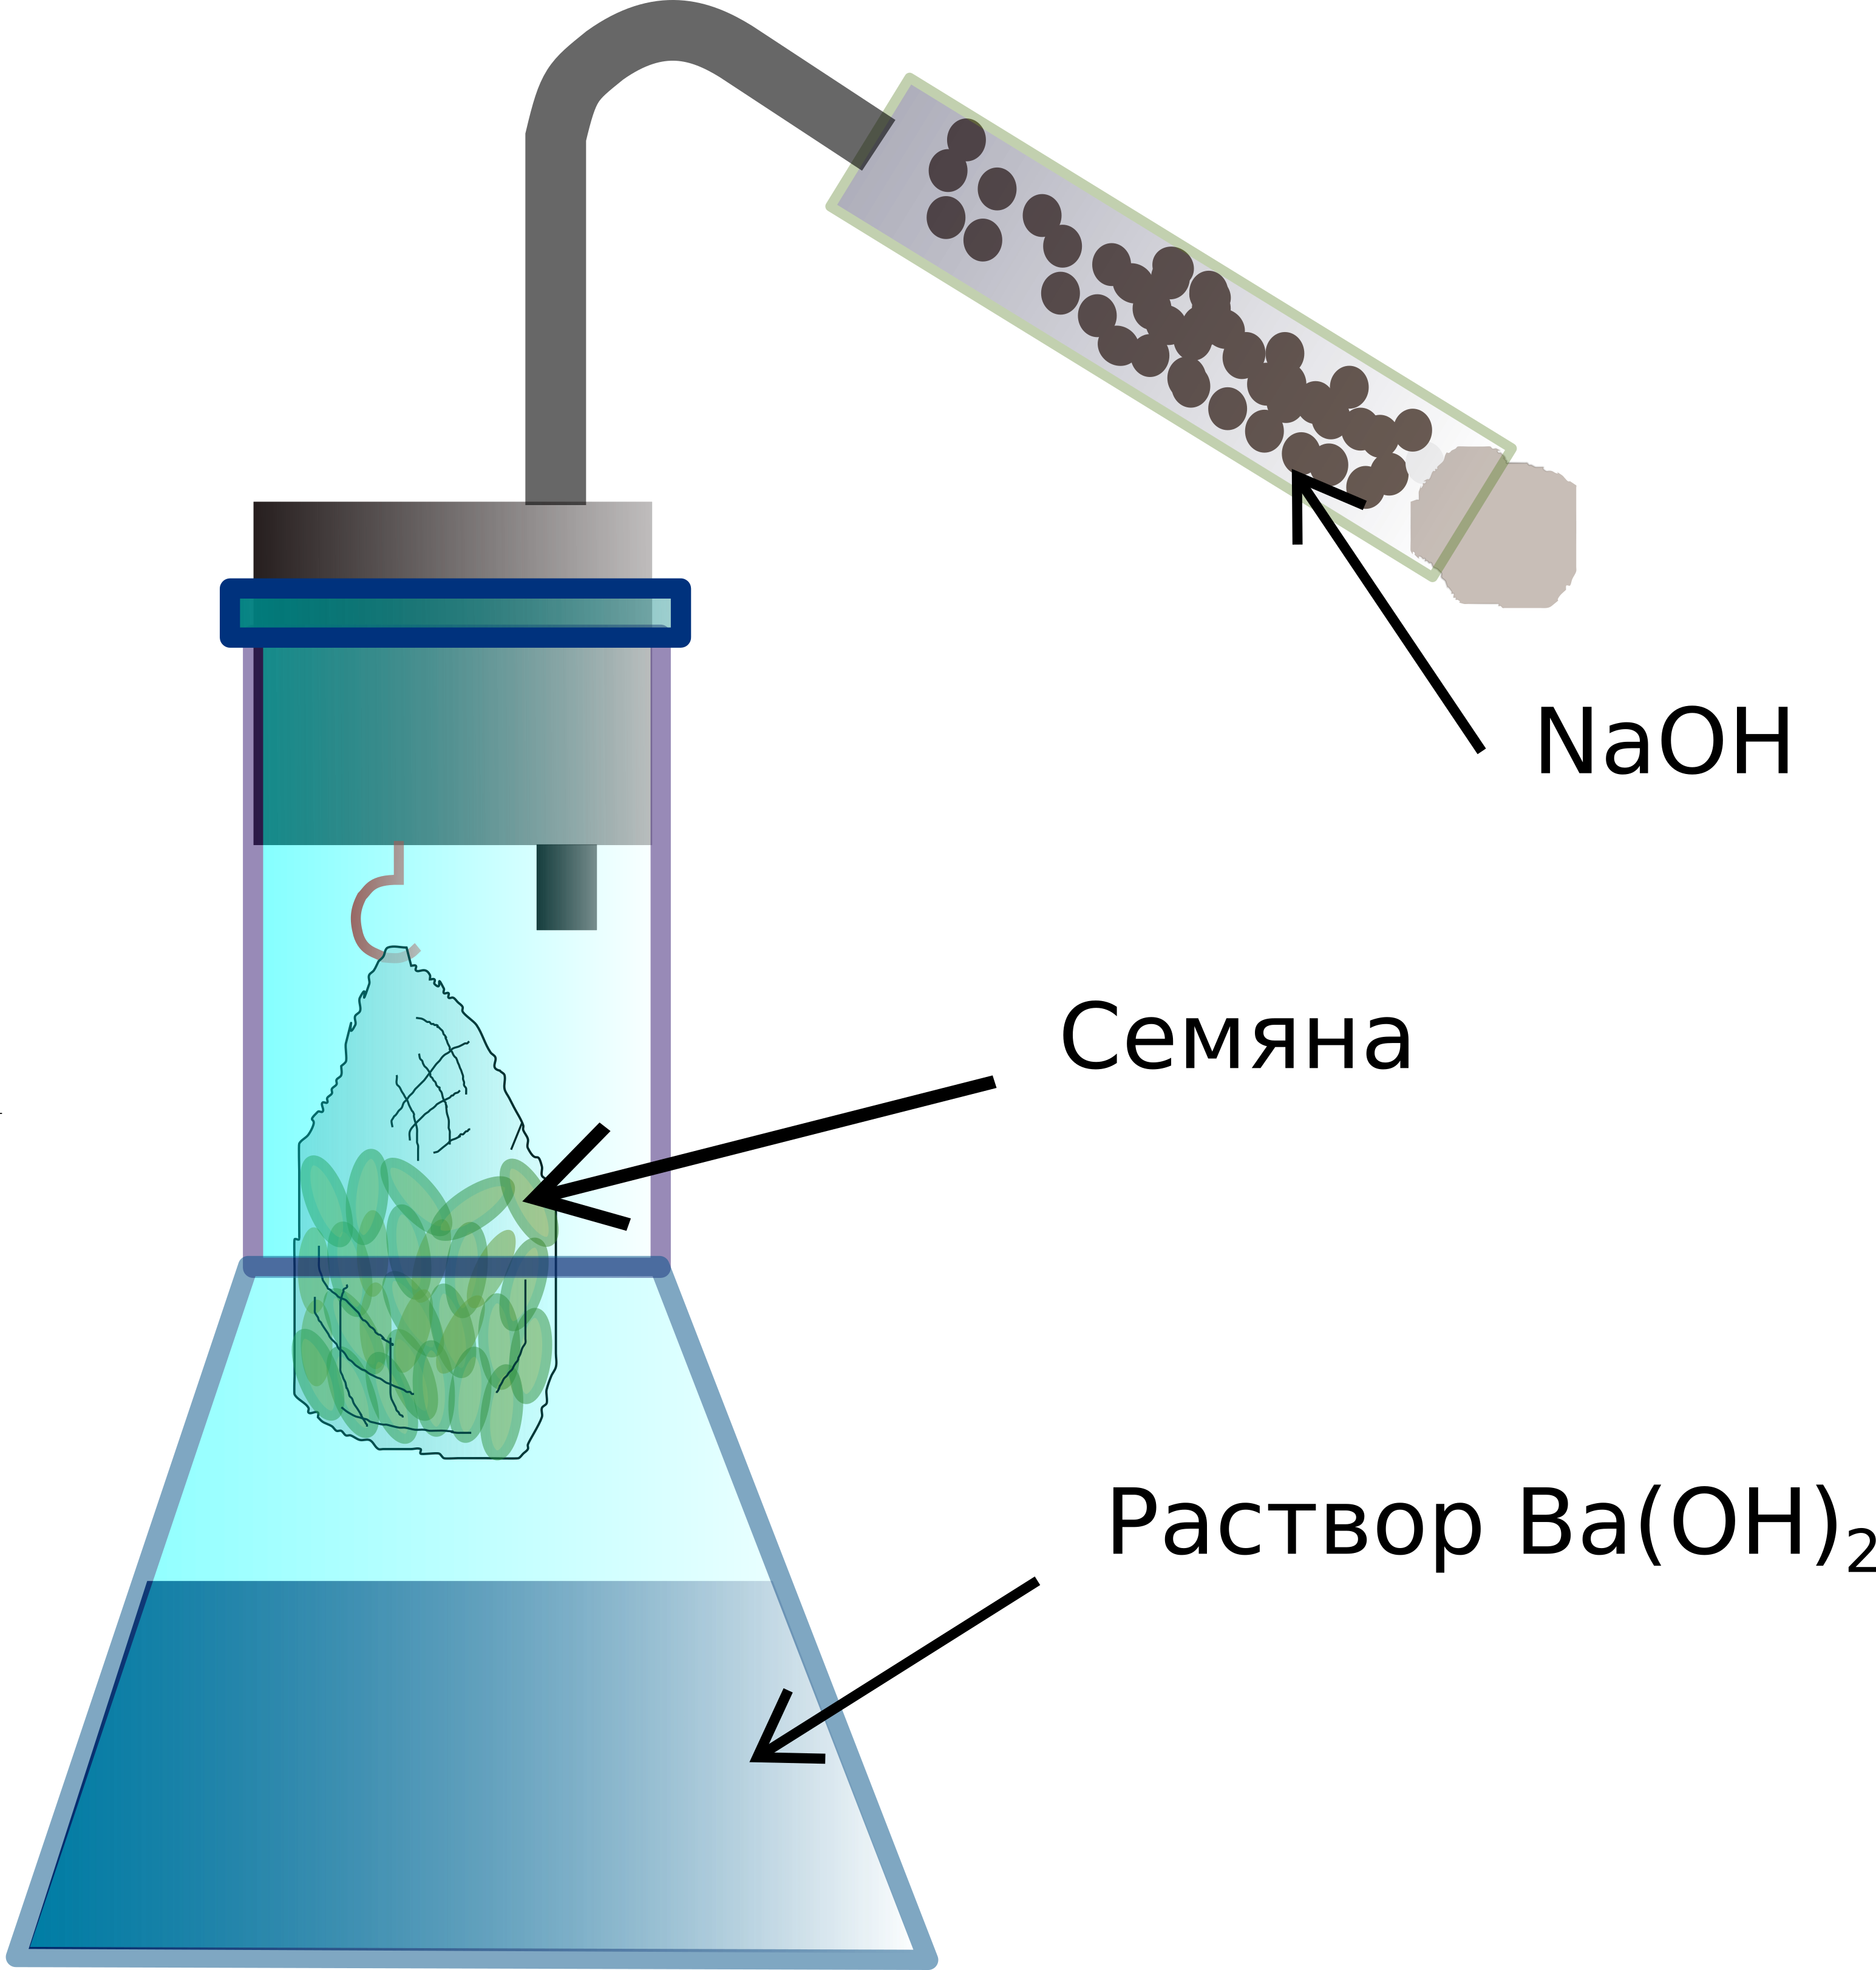
\includegraphics[width=0.5\linewidth]{pictures/breazing_colba}
\caption{Прибор для измерения интенсивности дыхания}
\label{breazing_colba}
\end{figure}
%%%%%%%%%%%%%%%%%%%%%%%%%%%%%%%%%%%%%%%%%%%%%%%%%%%%%%%%%%%%%%%%%%%%%%%%%%%%%%%%%%%%%%%%%%%%%%%%%%%%%%%%%%%

\paragraph*{}Оставьте обе колбы на 1 час при комнатной температуре, при этом содержимое колб периодически осторожно перемешивают, покачивая колбы. Это необходимо для того, чтобы разрушить плёнку углекислого бария, которая со временем образуется на поверхности баритной воды и препятствует поглощению.

\paragraph*{}Одновременно с первым опытом, проведите такой же опыт на семенах, выдержанных при температуре 30 градусов. 

\subsubsection{Определение интенсивности дыхания}

\paragraph*{}Через 1 час извлеките из колбы мешочек с семенами, а в саму колбу добавьте три капли фенолфталеина и оттитруйте барит 0,1 н до слабо-розового окрашивания, исчезающего от одной капли кислоты. Так же оттитруйте барит и в контрольной колбе. При проведении титрования колбы надо закрыть пробкой, через которую проходит кончик пипетки, присоединённой к бутылке с баритом\footnote{При титровании необходимо свести до минимума контакт баритной воды и воздуха так как баритная вода будет продолжать связывать углекислый газ воздуха во время титрования, что приведет к искажению результатов опыта}.

\paragraph*{}интенсивность дыхания семян рассчитывается по формуле \ref{baoh_titr}:

\begin{equation}
	\label{baoh_titr}
	J = \frac{(a-b)K.2,2}{n}
\end{equation}

\paragraph*{}Где \textit{a} и \textit{b} - количество 0,1 Н щавелевой кислоты, которая была израсходована на титрование барита в контрольном и опытном вариантах, мл; \textit{K} - поправка к титру 0,1 н раствора щавелевой кислоты; 2,2 - количество $CO_2$ мг, соответствующее 1 мл 0,1 Н раствора щавелевой кислоты; \textit{n} - масса сухих семян г 

\paragraph*{}Параллельно определите дыхание семян при 30 градусах. Результаты опыта запишите по форме.

\paragraph*{}\textbf{Сделайте вывод} о влиянии температуры на интенсивность дыхания.

\subsection*{Вопросы для самоконтроля}

	\begin{itemize}
		\item В чем заключается значение дыхания для живых организмов?
		\item Напишите балансовое уравнение дыхания;
		\item Какие факторы влияют на интенсивность дыхания?
		\item Для чего применяется метод титрования. В чем заключается его сущность? Какие типы титрования существуют?
		
	\end{itemize}
